\documentclass[11pt]{llncs}

\usepackage{calc, amssymb, amstext, amsmath}
\usepackage{boxedminipage, xspace, here, float}
\usepackage{epsfig, graphics, graphicx, xcolor, color, setspace, tabularx, multirow}
\usepackage[linewidth=1pt]{mdframed}
\usepackage{chngcntr} 
\usepackage[font={small}]{caption, subfig}
\usepackage{balance}

\usepackage{hyperref, url}
\usepackage{arydshln}
\usepackage{csquotes}
\usepackage{verbatim}
\usepackage{booktabs}
\usepackage{lscape}



\pdfcompresslevel=9
%\DeclareGraphicsExtensions{.png} 
\graphicspath{{img/}{svg/}} 

 
 
\usepackage{ifthen} 
\newboolean{showcomments} 
\setboolean{showcomments}{true} % toggle to show or hide comments
\ifthenelse{\boolean{showcomments}} 
  {\newcommand{\nb}[2]{
    \fcolorbox{gray}{yellow}{\bfseries\sffamily\scriptsize#1}  
    {$\blacktriangleright$#2$\blacktriangleleft$} 
   }
   \newcommand{\version}{\emph{\scriptsize$-$working$-$}}
  } 
  {\newcommand{\nb}[2]{} 
   \newcommand{\version}{}  
  }    
% for comments 
\newcommand\levi[1]{\nb{Levi}{\textcolor{teal}{#1}}}
\newcommand\tahira[1]{\nb{Tahira}{\textcolor{blue}{#1}}}

\newcommand{\etal}{\emph{et al.}\xspace}
\newcommand{\RE}{\textsc{Re}\xspace}
\newcommand{\ML}{\textsc{Ml}\xspace}


%\setlength{\textwidth}{13cm}
%\setlength{\textheight}{19cm}
% \setlength{\oddsidemargin}{1.1cm}  
% \setlength{\evensidemargin}{1.1cm}

%\newcommand{\newpar}[1]{\noindent
%\textbf{#1.}\hspace{0.3cm}
%}

\usepackage{inputenc} 
\inputencoding{utf8}

\begin{document} 
\frontmatter          % for the preliminaries
\mainmatter              % start of the contributions
\title{ \Huge \textbf{Extracting User Requirements from Social Media Using Machine Learning} }
\author{Tahira Iqbal}
\institute{
fortiss — An-Institut Technical University Munich, Germany \\
\email{iqbal@fortiss.org} 
}
\pagenumbering{gobble}
\maketitle
\newpage
\pagenumbering{arabic}

  
\section{Introduction}

Determining and managing users needs related to software and hardware is known as
Requirement Engineering (RE). RE is a key phase in the software development. In the past,
RE was considered only in the initial phase of software life cycle, e.g. waterfall model, and it was
not integrated into the remaining software development life cycle. As the time passed, software
development models evolved, and it became part of complete software development life
cycle.
Software systems are developed over millions of lines of code, a number of modules and
documents. The primary goal of the software system is to satisfy users by developing the
software that can meet their needs and expectations. This goal is achievable by applying
different methodologies and engineering techniques. One of the important factors is to understand and
identify the needs of users, also known as, software requirements. Software requirement
engineering is the process that helps to determine the requirements systematically to know
what functionalities the targeted system should have to fulfill users needs. Formally RE is
defined as \cite {Zave:1997} :\\
\textbf{ `` Requirements engineering is the branch of software engineering concerned with the real-world
goals for, functions of, and constraints on software systems. It is also concerned with the
relationship of these factors to precise specifications of software behavior, and to their evolution
over time and across software families.''} \\

	Software requirements plays a key role in the success of a project. In the USA, a survey was
conducted over 8380 projects by 350 companies to know the project failure rates. The report
 \cite{StandishReport} results showed only 16.2\% projects were completed successfully and one-half (52.7\%)
of projects met with challenges and were completed with partial functionalities, time delays and
over budget. Almost 31\% of the projects were never completed. The main cause told by the
executive managers was poor requirements engineering. The major problems were the lack of user
involvement (13\%), requirements incompleteness (12\%), changing requirements (11\%),
unrealistic expectations (6\%), and unclear objectives (5\%). \\

	 Software requirement engineering has mainly four phases; requirement elicitation, requirement
analysis, requirement documentation and requirement verification\cite{Kotonya:1998}. Requirement elicitation
\cite {Coughlan:2002} \cite {Zowghi2005}  helps to understand the stakeholder's needs, e.g. what features he wants in the software.
Requirement elicitation techniques are mostly derived from social sciences, organizational
theory, knowledge engineering and practical experience. For requirements elicitation, different
techniques exist in the literature that include interviews, questionnaires, and ethnography etc.
Requirement analysis \cite{Nuseibeh:2000} is the next step after requirement elicitation. In this phase, software
requirements are analyzed to check conflicts and consistency. It also makes
sure that the requirements are clear, complete and consistent. Furthermore, the agreed
requirements are documented. This documentation has a clear and precise definition of the
system functionalities. It also acts as an agreement between stakeholders and developers. These
functionalities and requirements are documented usually as diagrams, mathematical formulae
or natural languages. These documents are used and iterated until the end of the project.\\

	System requirements are classified into functional requirements (FR), non-functional requirements (NFR), user requirements, business
 requirements. Functional requirements are the system requirements that include the main
features and characteristics of the desired system. Non-functional requirements are the system
properties and constraints \cite{Davis:1993} \cite{Glinz}. NFRs set the criteria for judging the operation of the system such as performance, availability, and reliability etc. Business requirements are specified to address business objective, vision, and goal. It is defined at a higher level from organization or company and considered for designing the products. User requirements are the wish list for the system from users. User requirements are valuable for ensuring the system performs similarly to user needs.\\

\subsection {Machine Learning}
Machine learning (ML) is an emerging field of this era
and is a part of Artificial Intelligence (AI). It helped to solve complicated and hard problems in
software engineering efficiently \cite{Zhang2003}. ML mainly relies on the data and its algorithms learn
from existing datasets. It also helps to predict solutions for unseen problems. Automated learning
processes took great inspiration from human learning i.e. learning from examples. ML algorithms
have proved to have a significant impact in different fields e.g. business, medical, software
engineering, computer security, data and communication networks and others. For the leaning
process algorithm, another key factor are features. Features are the selected properties of a
problem that help in predicting the results. As an example, for a disease diagnostic software,
patient symptoms are the features.  List of symptoms is mapped to the particular disease. Now, if a new patient comes with some symptoms, the system would be able
to predict the disease by learning from the existing dataset. In addition, features help to abstract the complexities of the information
provided for learning. In short, a good selection of features leads to better and faster
learning.\\

	ML algorithms are divided into two major categories; supervised learning and unsupervised
learning \cite{Davis:1993} \cite{kotsiantis2007}. A third category is reinforcement learning which has been added at a
later stage. In supervised learning, data set is labeled. Response to a new input or query
is predicted after learning from the labeled data. All regression and classification
algorithms come under the umbrella of supervised learning e.g. Logistic Regression, Decision
Trees (DT), Support Vector Machine (SVM), Nearest Neighbors (NN), Naive Bayes (NB), Random
Forest and Artificial Neural Network (ANN) etc. \cite{lison2015introduction}. On the other hand, unsupervised learning used unlabeled data. It covers all clustering algorithms e.g. k-means clustering and
hierarchical clustering etc. A supervised classification algorithm learns from the recorded labeled data and on counterpart unsupervised finds similarities between the data and separates data into groups accordingly, assign a new label to each group. Several approaches leveraged a combination of both and known as semi-supervised learning. Semi-supervised learning is a class of supervised learning tasks and techniques that also utilize unlabeled data for training. It uses a small amount of labeled data with a significant amount of unlabeled data to build the predictive model.\cite{SemiSupervisedLearning} 
\section{Literature Review}
This section describes the current trends in RE and ML. It will define a few problems that have
been solved or automated using ML. Currently, I am working on a survey paper of RE and ML.
This literature includes only the related paper to the problem statement, which I have proposed in this
document. The full literature review is under progress.
\subsection{Requirement classification}
As per our on-going survey findings that we are writing, the most highlighted problem in RE
recently is requirement analysis. It deals with the classification of functional and non-functional
requirements. Requirements documents are usually written in natural language and
contain hundreds of requirements. It is hard and time-consuming to classify them manually.
These classifications are not limited to only FR and NFR, but also to the subcategories of NFR
and quality attributes. This problem area can be categorized on the basis of existing datasets in
the literature. In our categorization, we identify the following three classes of datasets:
\begin{itemize}
\item{App Stores}
\item{Social Media}
\item{Internal Application or Software}
\end{itemize}
\subsection{App Stores}
Millions of users share their reviews on app stores after downloading and using apps. They not only rate the apps but also write about the liked and disliked features. It is not easy to
find the requirements out of such a complex data. New features identification, classification of
FR and NFR, and summaries of the reviews for the improvements of an app is often done with ML
\cite{deocadez2017} \cite{lu2017automatic} \cite{maalej2015bug} \cite{jiang2014}. \\

	For the automated classification of FR and NFR, \cite{deocadez2017}  used a total of 932,338 online
reviews of the 40 top paid and free apps on appstores from top 10 different categories. Semi-supervised algorithm self- training, RASCO, Rel-RASCO for self-labeling is being used. This
semi supervision technique overcomes the manual annotation problem and shows that only
small amount of labeled data can achieve high accuracy. Naïve Bayes classification performs better than kNN, C4.5, and SMO.\\

	Another study on the classification of FR
and NFR was performed in \cite{lu2017automatic} on 6,696 raw user reviews from
iBook and 4400 raw user reviews from WhatsApp. It uses concept of
augmentation of user reviews and effectively improves user reviews classification results by
adding textual semantics to the sentences. The user reviews are augmented by several similar
words for better classification of results. The bagging algorithm outperformed Naïve Bayes and J.48.\\

	A classification method is produced in \cite{maalej2015bug} for identifying
bug reports and feature requests from user reviews. Total 146,057 reviews for 40 apps were
collected from Appstore and Google Play Store. For further experimentation, 4,400 reviews
are selected. The proposed model shows the upwards of 70 percent precision and 80 percent
recall could be obtained using multiple binary classifiers, as an alternative to a single multiclass
classifier. For the classification, binary Naive Bayes algorithm is used. The results show that
the commonly used NLP techniques such as stop word removal and lemmatization could
negatively affect the performance of this classification task.\\

	In the paper \cite{jiang2014}, the primary goal is to transform online reviews into evolutionary requirements.
Karplersky internet security 2011 from Amazon and mobile app of Tune-In Radio Pro V3.6
from the appstore are taken as dataset. The characteristic analysis of the reviews is
considered for the automated task analysis and software relation-based propagation approach
(SRPA) technique is used for the identification of opinion about common software features. Each set
manually labeled the potential software feature, opinion and the polarities in the reviews, and
then classify the reviews on the basis of relevant opinion semantics. For clustering, the opinion
expression network algorithm Grivan Newman (GN) is used in the proposed methods S-GN. The GN algorithm produces optimized number of clusters. For the second problem, the system helped the developer and proposed a set of related evolutionary requirements for the system.This problem in this study makes it more interesting by suggesting the relevant and essential
user requirements to a developer by adding polarization factor. That is not used
commonly in this domain.\\

\subsection{Social Media}
Social media e.g. Twitter and Facebook have become popular platforms to gather the
requirements from user posts. Users are sharing their new features requests, feedback and bug
report on social platforms. Previous studies \cite{Singer:2014} \cite{Prasetyo} \cite{Achananuparp:2012} in software engineering have applied different techniques to analyzed tweets contents related to software development. These tweets were posted by developers describing the relevant and irrelevant programming languages, libraries system methodologies tweets for software development. Our study is focused on getting user feedback for software application and mobile applications for obtaining user requirements. ML has been used to classify tweets into meaningful
categories like new requests and bugs etc. \cite{guzman2017} \cite{williams2017} . These classifications and the information
from these tweets helped the industry to know the user feedback for software improvements.\\

	ALERTme \cite{guzman2017} approach proposes for classifying, grouping and ranking tweets in software
evolution process. For this, a total of 68,108 tweets i.e., collection of two months of tweets about
Spotify, Dropbox, and Slack software dataset are used. The output is binary classification i.e.
improvement request or other. For the automated classification, supervised learning algorithm Multinomial Naïve Bayes is used.  
Further improvement requests are considered for the
grouping which helped to sort the request and summarize them accordingly. The major contribution helped to reduce human
effort to analyze each tweet for eliciting the requirements and knowing the issues of software. As the last step, these summaries and tweets are ranked by high
worthy tweets. A drawback of this study is the high number of manual annotations for labeling
the data as request or others. Besides, the majority voting scheme is being used to solve the
disagreements. Three annotators did this process, and it took around 13.5 hours for each
annotator to complete the task.\\

	The next study \cite{williams2017} classify and summarize the tweets. A total of 
4,000 tweets are randomly selected for ten different software. The proposed model
classifies them into bug, requirement, and spam using Naïve Bayes and SVM. The results
showed that 50\% of data contained useful technical feedback and achieved an average
classification F1 of 72\% using SVM that is better than state of the art in the literature  \cite{guzman2017}. The
reason is the feedback dedicated to technical stakeholders i.e. developer related tweets are
focused and analyzed. Tweets dataset is labeled manually. Different techniques with VSM and
NB are used. VSM is used for preprocessing e.g. stop word removing, sentimental analysis, stemming,
and Bag of words. However, the results show that these parameters do not
improve to help the results of ML algorithm for classification of the tweets. Unlike the political
tweets which are polarized and carry emotions, software tweets are neutral in nature.\\

\subsection{Internal Application or Software}
The third category is dealing with requirement classification using the software product data
i.e. written in Software Requirements Specification (SRS). It could be dataset for some interanl used software system. This data is composed of different software functional and nonfunctional
requirements.  The nonfunctional requirements have subcategories that include availability,
fault tolerance, legal, look and feel, maintainability, operational, performance, portability,
scalability, security and usability etc. This dataset is provided by the Requirement Engineering
(RE) conference and named as Quality attributes (NFR) dataset. The size of the total data set
has 625 requirements with 225 FR and rest with NFRs subcategories. \\

	For the automated classification of FR and NFR and identification of the subcategories of NFR \cite{kurtanovic2017}, support
vector machine (SVM) algorithm is used. The data is not equally distributed because of the small
number of requirements in NFRs subcategories, which are ignored. Data
under-sampling problem is solved by using external data i.e. user comment
dataset from the Amazon, and a hybrid approach is proposed with the new dataset. This
dataset contains performance and usability requirements. For the identification of specific
NFRs, proposed methodology achieve the highest precision and recall for security and
performance NFRs with ~92\% precision and ~90\% recall. \\

	Two main goals are targeted \cite{Abad},
first is classifying the FRs and NFRs, and second is an identification of NFR category. The data is
pre-processed as a first step. Feature co-occurrence and regular expression are used to increase
the weight of influential words used in NFR. The supervised learning algorithm J.48 DT is used
for classifying FRs and NFRs. For achieving the categorization or classification of NFR,
topic modeling using unsupervised algorithm LDA and BTM is applied. For the topic generation, the results show  that BNB works better than clustering, k-means, LDA, BTM. \\


	Another study for solving the same problem with NFR dataset with additional security dataset is conducted \cite{Dekhtyar}.
Software requirements are classified with the focus on security related requirements. ML algorithm
CNN with a specific setting in Tensor-Flow helped to achieve the goal and better results. In all
these classification problems, human input is involved for the annotation of the requirements.
Semi-supervision requires less human effort in labeling requirements than fully supervised
methods. The semi-supervised approach \cite{Casamayor} using Naïve Bayes resulted in accuracy rates
above 70\%, considerably higher than the results obtained with supervised methods using
standard collections of documents.
\section{Problem Statement}
Conventionally, software requirement elicitation and analysis are only limited to meetings,
interviews, and documented data etc. All the tasks are performed manually, requiring more
effort and time. With recent data trends from various sources, the user satisfaction and opinion
are more integrated into the industry. Recent studies mentioned in literature section have shown that the user analytics tools
and techniques are helping developers and practitioners to deal with a large number of user
feedback by filtering, classifying, and summarizing them, to decide what requirements and
features they should add, change or eliminate. Different ML algorithms have been used for
making it automated with different settings and parameters.\\

	 Most of the studies are using the app stores or Twitter data. A recent study has shown that the data from Twitter and app
stores reviews can complement each other \cite{Nayebi}.This study analyzed  97.1 \% cases mining tweets provided complementary information to developers about user 
feature request and bug report. Among all the apps 198 feature requests (22.48\%) and bug reports 246(12.98\%) were not reported in app store review. 
40.78 \% feature requests and bug reports across tweets and app reviews were common. These results showed that complementary data source 
gave better decision support. The use of
similar user discussion online platforms can give more knowledge to help achieve better results. 
This domain is not completly explored yet, and improvements can be done by using different
algorithms and techniques. \\

Also, the impact of these studies results in a real project is missing and
not discussed clearly. It is not researched and discussed in the literature that how these studies and techniques are helping and useful in the industry. For Example, if a developer is using application for getting user requirements from social media. How many user requirements were suggested by the proposed system and how many requirements were actually implemented and devolped. These results will explain is it useful or not to mine social media for gathering user requirements. In short, two primary goals or contributions can be seen as:\\
\begin{itemize}
  \item First is researching the hybrid data sources e.g. tweets, appstores, linkedin etc for user requirements for buidling a new app or for the next version of the exisiting app.
  \item Second is identifying the real impact and usefullness of mining social media results in the industry.
\end{itemize}

The related research questions are:\\

\textbf{RQ1: Can advanced classifiers or advances settings perform better than the ones used in the existing
literature?}\\
Out of various classifiers, it has been found in the literature that SVM and NB perform well for
short texts. Since the user reviews about software systems are short texts, these two algorithms
are usually preferred. However, it could be researched that how advanced classifiers or settings perform
in comparison to SVM and NB. The comparison could be drawn on the basis of the ability of a
classifier to process larger datasets, the processing time, complexity analysis and accuracy of
classification.\\

\textbf{RQ2: What would be the impact of using semi-supervised in
contrast to supervised learning?}\\
One of the problems with the classifiers usually used SVM and NB is that they fall into the
category of supervised learning. Supervised learning classifiers require a lot of human input as
they work on the basis of provided training data. The training data needs to be classified by
humans which is time consuming, particularly for large datasets such as the ones we are
discussing. In such scenarios, semi-supervised and unsupervised learning would require
less human input. Such techniques might decrease the efficiency, but for larger datasets, semi-supervised
might be less time consuming than supervised learning
techniques.\\

\textbf{RQ:3 How social network sites (Twitter, Facebook and LinkedIn etc.) and online discussion
forums (app stores and Amazon) reviews complement each other for developing the new
app or software?}\\
The importance of the end user involvement in today’s software is highlighted
in the literature. However, the reusability of this large dataset is not discussed and missing. The
addition of the social media data in the software development process in early stages can add
global and heterogeneous perspectives. As different people from diverse cultures all around the world are sharing reviews about app or software on social media. The benefit of the large dataset is to gather information
about the specific category and see what requirements users wished to have in both functional and
nonfunctional perspective. A developer or practitioner without enough requirements for the project
 can take benefit of the existing data knowledge for
 specific app and domain. It will give an additional set of requirements and features and
domain-specific knowledge for building the better system. I want to Implement this idea to a case
study to know the impact and enhancement of requirement that can be gained by this additional
data.

	Also, some similar features mapping can be exciting. For example, in \cite{Martens:2017} performed an initial study to observe the impact of emotional sentiment on app reviews as an informative feature and its pitfall. After deciding and experimentation on hybrid sources, some other informative features from one source to another can be improvized.\\

\textbf{RQ4: How useful are the social network sites (Twitter, Facebook, LinkedIn) and online
discussion forums (app stores, Amazon, google stores) reviews for requirement elicitation
and what works better?}\\
Users discuss software systems on numerous platforms including social media websites,
app stores, and online discussion forums etc. However, all the discussions do not contain
information specific to requirement engineering. Any information that doesn’t fall into the
category of features requests or bug reports generally is not of interest to us. Therefore, it is
necessary to evaluate the percentage of relevant information in each of these platforms. A
comparative study could be useful to evaluate which of these platforms contain more useful
information as compared to rest of the platforms. Also, the hybrid models containing different
sources e.g. twitter and Amazon reviews, Twitter, and app stores. What combination works better
and provide more features or bug report.\\

	The datasets obtained from online platforms are huge. The content shared by the users in al large number. However, the information would be more or less relevant to similar
functionalities of the application. Going through all the extracted dataset that is classified as
feature report or bug report would be humanly impossible. It is therefore imperative to
summarize the obtained information. The summarization should not only group similar requests
or bug reports, but also emphasize on the most discussed issues. For example, if there is a bug
with a camera filter, and is discussed various times, it should be emphasized in the same manner
to the developer, indicating that it requires more or immediate attention.\\

	In this area after classification and all experiments no study has shown what was the impact 
of their finding and how useful it was for devolper or practioneers. I want to perform some study with help of  casestudy that can help to identifying the impact
 of these finding in industry. The other missing feature in the literature is adaptability of the tool in the industry. For making
this concept more practical and useful in real life there should be some tool or plugin with
the entire features. I have to research the existing tool and their use in the industry for more
clarity. The ongoing survey disclosed the fact that tool is not available or if available only
taking data from one source. For this gap, we can develop the plugin. That plugin can be added
to the existing RE tools used in the industry.
\section{Proposed Methodology}
The basic focus of the current research is to extract feature requests and bug reports for popular
software systems and applications, as the discussions or user stories are readily available for
them. The classification is performed on the basis of applications, and not the specific
functionalities of these applications categories. However, there is not much benefit of it to the new
developers or developers of less popular systems. Since the functionalities in newer or less popular systems are more or less similar to the popular
applications, there could be a possibility that the information contained in the user stories of
popular applications can be made to use for newer systems. The proposed methodology
basically focusses on suggesting feature requests and bug reports on the basis of individual
functionalities of a software system and software category. Whenever a new developer wants to create a new
application, he selects the category for building his application. If devolper wants to see the new feature for his exisiting application he will specify the application.\\

	The database is populated based on the feedback from the classification and summarization
block. The purpose of the classification and the summarization block is to take input from the
existing social media and online platforms like Twitter, Facebook, App stores and LinkedIn etc.
So far only single study \cite{Nayebi} exist that takes data from two sources i.e. Twitter and app store.
Otherwise, the data from these sources were dealt separately. Different steps to be
performed are shown in Figure 1.

\begin{figure}
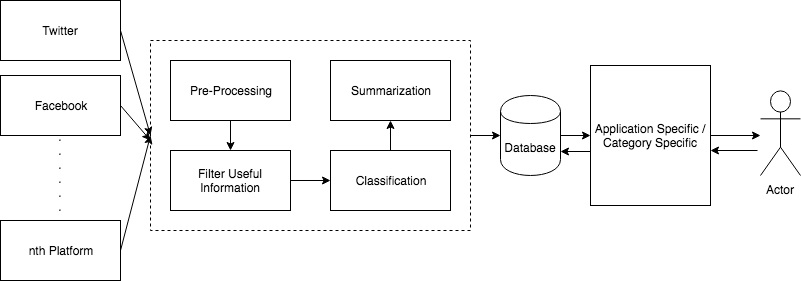
\includegraphics[width=\linewidth]{fig.png}
\caption{Block diagram of proposed methodology.}
\end{figure}

\textbf{Step 1 - Data Preprocessing: } The input data will be prepared for classification after preprocessing. This step will probably include tokenization, removal of stop words, stemming, etc. This step majorly depends on the chosen dataset combination, as different social media platforms have their own limitations.\\

\textbf{Step 2 –  Filter useful information: } This step will gather and filter the selected App or category description data. Each application has a description on app stores and on their Twitter or Facebook page. This description will be helpful to determine the main feature of an application as relevant information. Also, some behavior feature will be learned.  For example how much is the company responsive and replies to the customer. This description data will be filtered upon the user selection. It can also be used in next step as metadata.\\

\textbf{Step 3 –  Classification: } Not all user discussions will be useful for feature requests or bug reports extraction. Therefore, it is necessary to filter out useful information from the other. The semi-supervised algorithm will learn a classifier. That will classify the data into a feature request, bug reports, and other categories.\\

\textbf{Step 4 – Summarization: } Multiple discussions could be related to the same feature or bug.
Since the datasets extracted from the sources is so massive, going through the complete datasets
would be humanly impossible. The information needs to be summarized so that the similar type
of information can be seen together. In this ranking process will consider features from the different sources such as likes, share, user behavior, sentiment analysis etc. As our dataset will be multi sourced, different features and their impact will be researched on each dataset for future selection. As the last step, all information will be clustered using topic modeling algorithm. This will
give developers and practitioner an idea of which feature requests or bug reports are more emphasized and frequently discussed as compared to the rest.\\

	The main aim of the proposed methodology is to assist developers who want to develop a new
system or developers of a system with less number of users. With this technique, such
developers will be able to get the advantage of the user reported features requests and bug reports
from popular applications. Further, the information will be summarized on the basis of specific
functionalities. So, if a developer wants to include two functionalities that exist in WhatsApp,
and two functionalities that exist in Snapchat, he can easily see what are the feature requests
and bug reports individually for all of these functionalities. This will hopefully result in better
developed applications as required by users, quicker bug fixes even before the final release, and
better testing of the applications before and after release.

\subsection{User Interaction with the system:}
\begin{itemize}
\item{\textbf{Use Case 1:\\}}
 \underline {Name:} Getting requirements for building a new application\\
 \underline{Brief Description:} Actor wants to get user requirements for building a new application in a specified category e.g. sports, entertainment etc.\\
 \underline{Actors: } Devolpers, Requirement Analyst.\\
 \underline{Basic Flow:}
\begin {itemize}
\item{Actor will select the option for building a new application.}
\item{Actor will choose the category in which he wants to builds a new application}
\item{System will collect the online data related to the specified category.}
\item{System will apply data preprocessing on the collected data.}
\item{System will classify data as user requirement, bug repot and other.}
\item{System will provide a list of most influential and top ranked user requirements and bug reports in form of extractive summary.\\}
\end{itemize}
\item{\textbf{Use Case 2:\\}}

 \underline{Name:} Getting updated requirements for existing application\\
 \underline{Brief Description:} Actor wants to get user requirements for his existing application such as Facebook, YouTube etc.\\
 \underline{Actors: } Devolpers, Requirement Analyst.\\
 \underline{Basic Flow:}
\begin {itemize}
\item{Actor will select the option for the existing application.}
\item{Actor will choose his application from the list.}
\item{System will collect the online data related to the specific application. }
\item{System will apply data preprocessing on the collected data.}
\item{System will classify data as user requirement, bug repot and other.}
\item{System will provide a list of most influential and top ranked user requirements and bug reports in form of extractive summary.\\}
\end{itemize}

\item\textbf{ {Use Case 3:\\}}

 \underline {Name:} Getting updated requirements for existing application\\
 \underline{Brief Description:} Actor wants to get user requirements for his existing application such as Facebook, YouTube etc.\\
 \underline{Actors: } Devolpers, Requirement Analyst.\\
 \underline{Basic Flow:}
\begin {itemize}
\item{Actor will select the option comparison from the existing application}
\item{Actor will choose his application from the list.}
\item{Actor will choose applications for the comparison from the list.}
\item{System will collect relevant online data for the list defined by the user.}
\item{System will apply data preprocessing on the collected data.}
\item{System will classify data as user requirement, bug repot and other.}
\item{System will provide a list of most influential and top ranked user requirements and bug reports in form of extractive summary.}
\end{itemize}

\end{itemize}

\subsection{Evaluation:}
%\subsubsection {Evaluation\\}
One of the identified gaps in my research is the lack of evaluation for the existing studies. Most studies did not map their experiments result on the industry needs and impacts. That means the obtained results are similar to the manual study performed in the industry, if yes then how much? Also, how efficient results automated systems are providing to the users by considering the extra information and non-relevant information? I plan to perform this evaluation study as given below: \\
\begin {itemize}
\item{The first method to evaluate the results is to draw a comparison between two different versions of one application. The specific application data will be collected before the new version. All the requirements given by the proposed system will be matched in the new version. Each identified requirement exist in the new version or not will be checked manually.\\}
\item{The second method is the automated version of first method. For this two dataset before and after the new version will be compared. This method will compare which requirements  are mentioned by users in the first dataset i.e. before the new version. A tracability link for these requirements will be generated in the second dataset i.e. after new version. If users has stopped asking about these requirements after the release, we assumed that those requirements are now part of the application in the new version.\\}
\item{In the third method, I will perform an industrial case study that will investigate the difference in the developer requirements list result and my tool result list. The developer will mark the similar requirements in both results and give comments on  comparisons. From these results, we can see the correctness and efficiency of our system. This study will help to provide the beter insight of the comparison due to the comments. That will ultimately help to provide better evaluation.\\}
\end{itemize}
First and second casestudy has some threats to validity such as if requirement identified by my proposed system is not devolped in the new version due to some constraints e.g. orgnaizational policies, finance, scope of application etc. The third method will add the comments of devolper in the results for better anaylsis and more insight.
\subsection{Timelone for thesis:}
%\subsubsection{Timeline or thesis }
\begin{itemize}
\item{\textbf{ WP1: data collection}}
\begin{itemize}
\item{ Literature survey for finding related tools and technologies for data acquisition}
\item{ Data collection from appstores and social media platforms e.g. Twitter, Facebook pages, and Instagram pages etc.\\}
\end{itemize}

\item{\textbf{ WP2: dataset creation}}
\begin{itemize}
\item{ Applying NLP techniques for pre processing}
\item{ Identification of features}
\item{ Labeling datasets}
\item{ Formation of individual and hybrid datasets\\}
\item{ Conference Paper submission\\}
\end{itemize}

\item{\textbf{ WP3: Algorithm identification for classification}}
\begin{itemize}
\item{ Applying various ML algorithms on datasets from WP2}
\item{ Identifying suitable combinations for the hybrid dataset}
\item{ Identifying appropriate ML algorithm for each of the dataset\\}
\end{itemize}

\item{\textbf{ WP4: Algorithm identification for summarization}}
\begin{itemize}\item{ Identifying features for ranking of classified datasets}
\item{ Applying algorithms for summary of classified datasets}
\item{ Conference Paper submission\\}
\end{itemize}

\item{\textbf{ WP5: Evaluation}}
\begin{itemize}
\item{ Perform case study1}
\item{ Perform case study for the automated analysis for the app versions} 
\item{ Results analysis of case studies}
\item{ Research Paper submission\\}
\end{itemize}

\item{\textbf{ WP6: Final submission}}
\begin{itemize}
\item{ Thesis Writing and submission}
\end{itemize}
\end{itemize}


% Please add the following required packages to your document preamble:
% \usepackage{graphicx}
\begin{table}[]

\resizebox{15cm}{2.5cm}{%
\begin{tabular}{|c|l|c|c|}
\hline
\textbf{Workpackage}                             & \multicolumn{1}{c|}{\textbf{Description}}                                                                                                                                                                                                              & \textbf{Start Date} & \textbf{End Date} \\ \hline
WP1: Data collection                             & \begin{tabular}[c]{@{}l@{}}1.1	Literature survey for finding related tools and technologies for data acquisition \\  1.2	Data collection from appstores and social media platforms e.g. Twitter, Facebook pages, and Instagram pages etc.\end{tabular} & 01/09/18            & 30/11/18          \\ \hline
WP2: Dataset creation                            & \begin{tabular}[c]{@{}l@{}}2.1 Applying NLP techniques for pre processing\\ 2.2 Identification of features\\ 2.3 Labeling datasets\\ 2.4 Formation of individual and hybrid datasets\end{tabular}                                                      & 01/12/18            & 30/04/19          \\ \hline
WP3: Algorithm identification for classification & \begin{tabular}[c]{@{}l@{}}3.1 Applying various ML algorithms on datasets from WP2 \\ 3.2 identifying suitable combinations for the hybrid dataset\\ 3.3 Identifying appropriate ML algorithm for each dataset\end{tabular}                            & 01/05/19            & 30/11/19          \\ \hline
WP4: Algorithm identification for summarization  & \begin{tabular}[c]{@{}l@{}}4.1 Identifying features for ranking of classified datasets \\ 4.2 Applying algorithms for the summary of classified datasets\end{tabular}                                                                                  & 01/12/19            & 30/6/20           \\ \hline
WP5: Evaluation                                  & \begin{tabular}[c]{@{}l@{}}5.1 Perform case study in the industry\\ 5.2 Perform case study for the automated analysis for the app versions.\\ 5.3 Results analysis of case studies.\end{tabular}                                                       & 01/07/20            & 28/02/21          \\ \hline
WP6:Thesis Writing                               & 6.1 Thesis writing and final submission                                                                                                                                                                                                                & 01/01/21            & 31/08/21          \\ \hline
\end{tabular}
}
\caption{Timeline for Thesis}
\end{table}
\begin{comment}
\begin{table}[]
\begin{tabular}{|p{3.5cm}|p{6.5cm}|p{2cm}|p{2cm}|}
\hline
\textbf{Workpackage}                             & \multicolumn{1}{c|}{\textbf{Description}}                                                                                                                                                                                                              & \textbf{Start Date} & \textbf{End Date} \\ \hline
WP1: Data collection                             & \begin{tabular}{p{6.5cm}}1.1	Literature survey for finding related tools and technologies for data acquisition \\  1.2	Data collection from appstores and social media platforms e.g. Twitter, Facebook pages, and Instagram pages etc.\end{tabular} & 01/09/18            & 30/11/18          \\ \hline
WP2: Dataset creation                            & \begin{tabular}{p{6.5cm}}2.1 Applying NLP techniques for pre processing\\ 2.2 Identification of features\\ 2.3 Labeling datasets\\ 2.4 Formation of individual and hybrid datasets\end{tabular}                                                      & 01/12/18            & 30/04/19          \\ \hline
WP3: Algorithm identification for classification & \begin{tabular}{p{6.5cm}}3.1 Applying various ML algorithms on datasets from WP2 \\ 3.2 identifying suitable combinations for the hybrid dataset\\ 3.3 Identifying appropriate ML algorithm for each dataset\end{tabular}                            & 01/05/19            & 30/11/19          \\ \hline
WP4: Algorithm identification for summarization  & \begin{tabular}{p{6.5cm}}4.1 Identifying features for ranking of classified datasets \\ 4.2 Applying algorithms for the summary of classified datasets\end{tabular}                                                                                  & 01/12/19            & 30/6/20           \\ \hline
WP5: Evaluation                                  & \begin{tabular}{p{6.5cm}}5.1 Perform case study in the industry\\ 5.2 Perform case study for the automated analysis for the app versions.\\ 5.3 Results analysis of case studies.\end{tabular}                                                       & 01/07/20            & 28/02/21          \\ \hline
WP6:Thesis Writing                               & 6.1 Thesis writing and final submission                                                                                                                                                                                                                & 01/01/21            & 31/08/21          \\ \hline
\end{tabular}
\end{table}%
\end{comment}

\begin{comment}
\begin{itemize}

\item{As a first step user will choose either he wants to build a new version of an existing application or a new application. Also, the user will determine that he wants to analyze specific application such as Facebook, chrome etc. 
or specific application category such as books, photo and video, news etc.}
\item{In the second step, some behavioral and main features of the application will be learned from the provided description on applications pages and app stores.}
\item{In the next step, data will be gathered based on the first step for preprocessing. This step output the clean data for further steps.}
\item{After preprocessing, data will be classified into categories based on user choice in the first step.}
\item{In the last step, most influential and top-ranked requests (reviews, Tweets etc) will be provided as a user requirement or main feature according to the user selected choice.}

\end{itemize}
\end{comment}


\section{Support in Fortiss}

One research project Center for code Excellence (CCE) can be considered good support in Fortiss. CCE has one part named as "Recognize and analyze trends" in which data will be collected from social media such as Twitter, and stack overflow. The collected data will be analyzed for prediction of future technology trend. I can start implementing my first task of the proposed solution and perform data analysis. For CCE project our implementations for data analysis can be seen as a common point. Furthermore, both side can improvize techniques according to their own needs and perspectives. Till now we both have to gather data from Twitter for analysis. However, the dataset for both of us will be different.\\  

	The other support is Dr.Levi Lucio due to his research interest in RE and ML. I am submitting a conference paper with him at the end of this week. Currently, one in-house fortiss project "User Modelling and User-Adaptive Interaction for Open Source Software Development Environment" is also under discussion. The main idea for my involvement in this project to get some hands-on experience and gaining a new research insight into my research. I will start working on the user research and analysis part. This project mainly deals with requirements on user needs, use case definition and requirements mapping and modeling user behavior and skills. This project will also help me to understand my future research integration and collaboration in AF3.\\ 
	
	The other support is from the OCPS project. It is a requirement for OCPS project to do secondments. Secondments are two visits in other labs for research collaboration. After the completion of the above two project collaborations, I am planning to go for my first secondments.Where I will target those labs which are researching the same domain, and I can collaborate on my work with them.





 
\bibliographystyle{unsrt} 
\bibliography{./ml_req} 

\end{document}
